\section{Experiments}
In this section, we present the results of our experiments.
We first describe end-to-end use cases of \sys measuring accuracy and end-to-end runtime.
Then, we present a series of micro-benchmarks that evaluate each of the modules of \sys.

\subsection{Baselines and Methods}
To the best of our knowledge, there does not exist a comparable general purpose ML+Data Cleaning system to \sys in industry or academia.
We evaluate \sys against a number of baseline approaches inspired by solutions proposed in literature. 

\vspace{0.25em}\noindent\textbf{No Cleaning: } We train a model without any modification to the training or test data.

\vspace{0.25em}\noindent\textbf{Quantitative Only: } We train a model where only quantitative outliers in both training and test are imputed with a mean value. 

\vspace{0.25em}\noindent\textbf{Integrity Constraint: } We train a model where integrity constraints are corrected using a statistical distortion minimization metric as in~\cite{prokoshyna2015combining}.

\vspace{0.25em}\noindent\textbf{Quantitative + IC + Default Value: } We train a model where both quantitative and qualitative violations are corrected with a single action to impute the mean value (numerical) or mode value (categorical/string).

\vspace{0.25em}\noindent\textbf{Best Single: } We run \sys for $B=1$ and identify the best single data cleaning operation.

\vspace{0.25em}\noindent\textbf{Worst Single: } We run \sys for $B=1$ and identify the worst single data cleaning operation.

\vspace{0.25em}
In all of our experiments, we used standard classification models and featurization techniques from Python \textsf{sklearn}.
The classifiers were trained in Python 2.7 and timing experiments were run on an Amazon EC2 m4.16xlarge instance\footnote{64 virtual cpus and 256 GiB memory}.
To avoid overfitting, we carefully designed the accuracy evaluation experiments for \sys.
We use a ``doubly'' held out test dataset to address this problem, i.e., the test dataset that we use to optimize \sys is different from a completely unseen test dataset which is used to evaluate prediction accuracy.

\subsection{ML Competition Datasets}
We downloaded 8 ML datasets used in Kaggle competitions and benchmarks in the UCI ML repository. The datasets are described below with brief descriptions and a description of the data errors:

\reminder{TODO Write Description}

\subsection{Data Analytics}
We applied \sys to two raw datasets

\reminder{TODO Write Description}

\subsection{Company X Experiments}
We applied \sys to three datasets from Company X.

\reminder{TODO Write Description}


\begin{table*}[t]
\centering
\label{my-label}
\begin{tabular}{|l|r|r|r|r|r|r|r|r|r|}
\hline
ML Competition& NC & Q &	IC & Q+IC &	Best-1 &	Worst-1 &	BC-3 & BC5 & Rel. Improvement\\
\hline
USCensus	&0.85&	0.82&	0.86&	0.84&	0.87&	0.79&	0.88&	\blue{0.91} & +4.5\% \\
Emergency &	0.67&	0.72&	0.67&	0.72&	0.72&	0.66&	0.72&	\blue{0.75} & +4.7\%\\
Sensor	&0.92&	0.84&	0.93&	0.89&	0.92&	0.8&	\blue{0.94}&	0.94 & +1.3\%\\
NFL	&0.74&	0.74&	0.76&	0.75&	0.76&	0.74&	0.79&	\blue{0.82}& +5.1\%\\
EEG	&0.79&	0.82&	0.79&	0.83&	0.83&	0.7&	0.85&	\blue{0.89}& +6.8\%\\
Titanic	&0.83&	0.72&	0.83&	0.76&	0.83&	0.69&	0.83&	\blue{0.84}& +1.1\%\\
Housing	&0.73&	0.76&	0.73&	0.77&	0.77&	0.65&	\blue{0.81}&	0.76& +5.1\% \\
Retail	&0.88&	0.88&	0.91&	0.91&	0.91&	0.87&	0.94&	\blue{0.95}& +4.3\% \\
\hline
\hline
Data Analytics & NC & Q &	IC & Q+IC &	Best &	Worst &	BC-3 & BC5 & Rel. Improvement\\
\hline
FEC  & 0.62 & 0.53 & 0.61 & 0.57 & 0.71 & 0.51 & 0.74 & \blue{0.77} &  +8.4\% \\
Restaurant (Multiclass) & 0.42 & 0.42 & 0.58 & 0.68 & \blue{0.62} & 0.36 & 0.61 & 0.60 & (1.61)\% \\
\hline
\hline
Company X & NC & Q &	IC & Q+IC &	Best &	Worst &	BC-3 & BC5 & Rel. Improvement\\
\hline
Dataset 1 & & & & & & & & &\\
Dataset 2 & & & & & & & & &\\
Dataset 3 & & & & & & & & &\\
\hline
\end{tabular}
\caption{This table presents end-to-end accuracy results for each of the experimental datasets for \sys and alternatives. The results presented describe standard classification accuracy.}
\end{table*}

\subsection{Micro-Benchmarks}






\iffalse
\begin{figure}[t]
% \vspace{-5pt}
\centering
 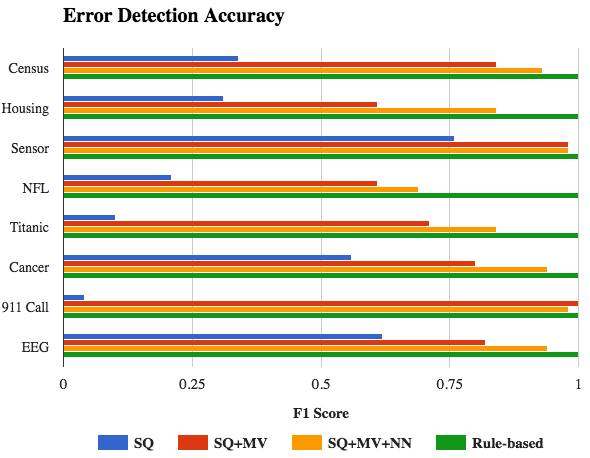
\includegraphics[width=\columnwidth]{figures/exp1-bar.png}
 \caption{On 8 Machine Learning datasets, we evaluated the F1 score of different error detection techniques. (SQ) returns all values above 5 standard deviations from the mean. (SQ+MV) additionally applies heuristics to detect missing values. (SQ+MV+NN) additionally uses a Neural Network to find anomalous correlations between attributes. A single hyperparameter setting was used across all datasts. While SQ on its own performs poorly, SQ+MV+NN approaches the performance of the programatic rule-based approach--but without requiring a user to write the program.
 \label{fig:error}}
\end{figure}

\subsection{Initial Experiments}
To explore this question, we downloaded 8 benchmark datasets previously used in Machine Learning competitions. These datasets varied in size from 1460 records to 928,991 records.
We programatically cleaned these datasets up front through manual inspection and taxonomized the errors that we found (Figure \ref{fig:error}).
These datasets were already structured but had attribute errors, outliers, and inconsistent coding.

Confirming the results of Abedjan et al.~\cite{DBLP:journals/pvldb/AbedjanCDFIOPST16}, we found that a 
purely quantitative approach does not perform well in comparison to the rule-based approach on these datasets.
However, results are significantly improved when combined with heuristics that detect missing values. 
The performance gap is even further reduced when the detector additionally uses a Neural Network to learn how attributes correlate with each other, and detect anomolous correlations.

It is important to emphasize that these datasets represent a very specific domain, i.e., structured training datasets for ML.
The datasets are already in a structured schema and the only thing that an analyst has to worry about is handling inconsistent attribute values.
Presumably these datasets were also previously cleaned and extracted before they were publicly released.
Our initial experiment showed that for this class of datasets, reasonably accurate error detection is possible with minimal supervision and tuning.

\vspace{0.5em}
\noindent\textbf{Common Cleaning Patterns: }  If we can enumerate much of the errors in the dataset, the natural next question is whether we can automatically synthesize code to handle these errors. Since these datasets are publicly available, we surveyed ML code on github to understand how developers generally handled the issues in the particular datasets. The interesting insight is that data cleaning before ML model training has different design patterns that typical relational data cleaning. We found three common operations: (1) \emph{Feature Imputation. } impute the erroneous entry with a sensible default (consistent null symbol, mean value, most frequent value),  (2) \emph{Label Imputation. } when asked to predict a label for a dirty record return a null prediction or the most frequent label, and (3) \emph{Removal. } remove a dirty record from the training dataset. For each of the errors detected there are three options, and the the problem is select one of the three options in each case as to maximize the prediction accuracy.
\fi